\chapter{Crescent}

\vspace{\baselineskip}

\begin{paracol}{2}

\begin{enumerate}
    \item Start travelling towards Crescent
\end{enumerate}

\switchcolumn
\begin{misc}{Path to Crescent}
    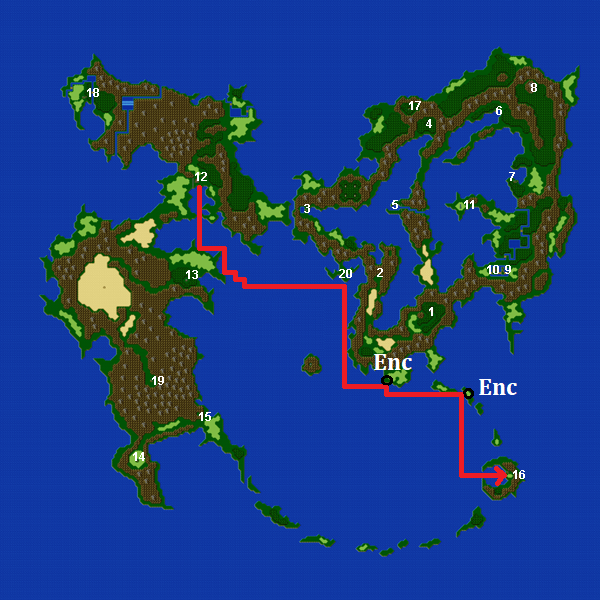
\includegraphics[scale=0.8]{../Graphics/Maps/2. To Crescent.png}
\end{misc}

\switchcolumn*
\begin{enumerate}[resume]
    \item Disembark at the following landmass
\end{enumerate}

\switchcolumn
\begin{steproute}{First Black Flame x5}
    \insertStep{../Graphics/Steps/59. Crescent Enc 1.jpg}
\end{steproute}

\switchcolumn
\begin{encounter}{Black Flame x5}
	\varwb
	\begin{notes}
		\item \encounterHl{Don't flee buffer}
		\item \encounterHl{Flame Scroll (\pointUp)}
	\end{notes}
	\begin{round}{1}
		\faris \leftCommand{\throw} \then \flameScroll
	\end{round}
	\varwe
\end{encounter}

\begin{menu}{After the First Black Flame Encounter}
    \varwb
    \begin{jobMenu}
        \lenna Time Mage \textbf{(\pointDown)(\pointRight)} \optimize
    \end{jobMenu}
    \begin{itemMenu}
        \potionMenu \ally{If necessary}
    \end{itemMenu}
    \varwe
\end{menu}

\begin{enumerate}[resume]
    \item Stop by at this island
\end{enumerate}

\switchcolumn
\begin{steproute}{Second Black Flame x5}
    \insertStep{../Graphics/Steps/60. Crescent Enc 2.jpg}
\end{steproute}

\switchcolumn
\begin{encounter}{Black Flame x5}
	\varwb
	\begin{notes}
		\item \encounterHl{Don't flee buffer}
		\item \encounterHl{Thunder Rod is already equipped}
	\end{notes}
	\begin{round}{1}
		\faris Defend
        \bartz Defend
        \lenna Item \then \battleGroup{\thunderRod} \then Break
	\end{round}
	\varwe
\end{encounter}

\switchcolumn
\begin{steproute}{Before Crescent}
    \insertStep{../Graphics/Steps/61. Crescent 1.jpg}
\end{steproute}

\switchcolumn
\begin{enumerate}[resume]
    \item Enter Crescent
\end{enumerate}

\end{paracol}